\documentclass{beamer}

\usetheme[progressbar=frametitle]{metropolis}
\usepackage{appendixnumberbeamer}
\usepackage{booktabs}
\usepackage{amsmath}
\usepackage{amssymb}
\usepackage{tcolorbox}
\usepackage{adjustbox}
\definecolor{metropolisblue}{RGB}{39, 59, 94}
\setbeamersize{text margin left=0.5cm,text margin right=1cm}

\newcommand{\data}{\mathcal{D}}
\newenvironment{myitemize}{%
\begingroup
    \setbeamercolor{itemize item}{parent=structure}
    \setbeamercolor{alerted text}{fg=black}
    \setbeamercolor{itemize/enumerate body}{fg=white}
    \begin{itemize}[<alert@+->]
}{
    \end{itemize}
\endgroup
}

% Begin document
\begin{document}

% Title page
\title{Bayesian Logistic Regression}
\author{Zeel B Patel, Nipun Batra}
\date{\today}
\institute{IIT Gandhinagar}
\maketitle


\begin{frame}{Outline}
    \tableofcontents
\end{frame}

% Section 1
\section{MLE}

\begin{frame}{Data}
    \begin{figure}
        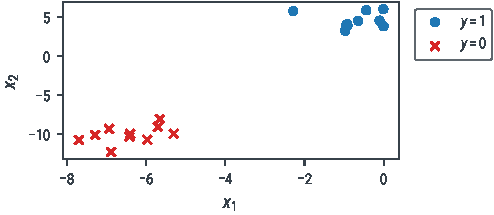
\includegraphics[]{../figures/bayesian-logistic-regression/data.pdf}
    \end{figure}
    \pause
    \begin{minipage}[t]{0.5\textwidth}
        \begin{table}
            \begin{tabular}{rrr}
                \toprule
                x1    & x2     & y   \\
                \midrule
                -5.97 & -10.68 & 0   \\
                -0.44 & 5.90   & 1   \\
                -0.97 & 3.27   & 1   \\
                ...   & ...    & ... \\
                \bottomrule
            \end{tabular}
        \end{table}
    \end{minipage}
    \hfill
    \pause
    \begin{minipage}[t]{0.4\textwidth}
        \begin{align*}
            \data & = \{(\boldsymbol{x}_i, y_i)\}_{i=1}^N \\
                  & = \{X, \boldsymbol{y}\}
        \end{align*}
    \end{minipage}

\end{frame}

\begin{frame}{Likelihood}
    \begin{align*}
        \onslide<1->{p(\data | \boldsymbol{\theta}) = p(\boldsymbol{y} | X, \boldsymbol{\theta})     & = \prod_{i=1}^N p(y_i | \boldsymbol{x}_i, \boldsymbol{\theta})}                                                                                                                                        \\
        \onslide<2->                                                                             {   & = \prod_{i=1}^N \text{Bernoulli}\left(\boldsymbol{\sigma}\left(\boldsymbol{\theta}^T\boldsymbol{x}_i\right)\right)  \;\;\;\;\left[\boldsymbol{\sigma}(x) = \frac{1}{1 + e^{-x}} \right]}               \\
        \onslide<3->                                                                               { & = \prod_{i=1}^N \boldsymbol{\sigma}\left(\boldsymbol{\theta}^T\boldsymbol{x}_i\right)^{y_i} \left(1 - \boldsymbol{\sigma}\left(\boldsymbol{\theta}^T\boldsymbol{x}_i\right)\right)^{1 - y_i}}          \\
        \onslide<4->{\log p(\boldsymbol{y} | X, \boldsymbol{\theta})                                 & = \sum_{i=1}^N y_i \log \boldsymbol{\sigma}\left(\boldsymbol{\theta}^T\boldsymbol{x}_i\right) + (1 - y_i) \log \left(1 - \boldsymbol{\sigma}\left(\boldsymbol{\theta}^T\boldsymbol{x}_i\right)\right)}
    \end{align*}

\end{frame}

\begin{frame}{MLE}
    \begin{align*}
        \onslide<1->{- \log p(\data | \boldsymbol{\theta})                                              & = - \sum_{i=1}^N y_i \log \boldsymbol{\sigma}\left(\boldsymbol{\theta}^T\boldsymbol{x}_i\right) - (1 - y_i) \log \left(1 - \boldsymbol{\sigma}\left(\boldsymbol{\theta}^T\boldsymbol{x}_i\right)\right)}                                                                          \\
        \onslide<2->{\frac{\partial}{\partial \boldsymbol{\theta}} -\log p(\data | \boldsymbol{\theta}) & = -\sum_{i=1}^N y_i \frac{\boldsymbol{\sigma}\left(\boldsymbol{\theta}^T\boldsymbol{x}_i\right)\left(1 - \boldsymbol{\sigma}\left(\boldsymbol{\theta}^T\boldsymbol{x}_i\right)\right)}{\boldsymbol{\sigma}\left(\boldsymbol{\theta}^T\boldsymbol{x}_i\right)} \boldsymbol{x}_i}   \\
        \onslide<3->{                                                                                   & \quad - (1 - y_i) \frac{\boldsymbol{\sigma}\left(\boldsymbol{\theta}^T\boldsymbol{x}_i\right)\left(1 - \boldsymbol{\sigma}\left(\boldsymbol{\theta}^T\boldsymbol{x}_i\right)\right)}{1 - \boldsymbol{\sigma}\left(\boldsymbol{\theta}^T\boldsymbol{x}_i\right)} \boldsymbol{x}_i} \\
        \onslide<4->{                                                                                   & = -\sum_{i=1}^N y_i \left(1 - \boldsymbol{\sigma}\left(\boldsymbol{\theta}^T\boldsymbol{x}_i\right)\right) \boldsymbol{x}_i - (1 - y_i) \boldsymbol{\sigma}\left(\boldsymbol{\theta}^T\boldsymbol{x}_i\right) \boldsymbol{x}_i}                                                   \\
        \onslide<5->{                                                                                   & = -\sum_{i=1}^N \left(y_i - \boldsymbol{\sigma}\left(\boldsymbol{\theta}^T\boldsymbol{x}_i\right)\right) \boldsymbol{x}_i}
    \end{align*}
\end{frame}

\begin{frame}{MLE}
    \begin{align*}
        \onslide<1->{X^T (\boldsymbol{\sigma}(X \boldsymbol{\theta}) - \boldsymbol{y}) & = 0}                                                                                       \\
        \onslide<2->{X^T \boldsymbol{\sigma}(X \boldsymbol{\theta})                    & = X^T \boldsymbol{y}}                                                                      \\
        \onslide<3->{\frac{1}{1 + e^{-X \boldsymbol{\theta}}}                          & = \boldsymbol{y}}                                                                          \\
        \onslide<4->{X \boldsymbol{\theta}                                             & = \log \left(\frac{\boldsymbol{y}}{1 - \boldsymbol{y}}\right)}                             \\
        \onslide<5->{\boldsymbol{\theta}_{MLE}                                         & = \left(X^T X\right)^{-1} X^T \log \left(\frac{\boldsymbol{y}}{1 - \boldsymbol{y}}\right)}
    \end{align*}
    \onslide<6->{
        However, $\log \left(\frac{\boldsymbol{y}}{1 - \boldsymbol{y}}\right)$ is undefined when $y_i = 0$ or $y_i = 1$, which is always the case.}
\end{frame}


\begin{frame}{MLE}
    \begin{itemize}
        \item There is no closed form solution for $\boldsymbol{\theta}_{\text{MLE}}$. So, we have to use gradient descent.
    \end{itemize}
    \pause
    \begin{figure}
        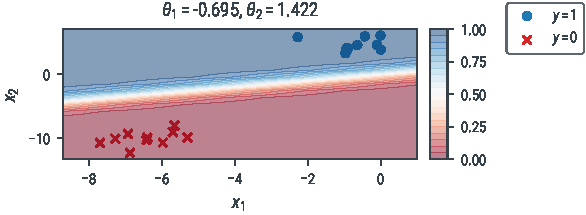
\includegraphics[]{../figures/bayesian-logistic-regression/mle.pdf}
    \end{figure}

\end{frame}

\section{MAP}

\begin{frame}{Prior}
    \begin{itemize}
        \item We may use a Gaussian prior on $\boldsymbol{\theta}$.
    \end{itemize}

    \begin{equation*}
        p(\boldsymbol{\theta}) = \mathcal{N}(\boldsymbol{\theta} | 0, \sigma^2)
    \end{equation*}

\end{frame}

\begin{frame}{Log Joint}
    \begin{align*}
        \log p(\boldsymbol{\theta}, \boldsymbol{y} | X) & = \log p(\boldsymbol{y} | X, \boldsymbol{\theta}) + \log p(\boldsymbol{\theta})                                                                                                                       \\
                                                        & = \sum_{i=1}^N y_i \log \boldsymbol{\sigma}\left(\boldsymbol{\theta}^T\boldsymbol{x}_i\right) + (1 - y_i) \log \left(1 - \boldsymbol{\sigma}\left(\boldsymbol{\theta}^T\boldsymbol{x}_i\right)\right) \\
                                                        & \quad  - \frac{1}{2} \frac{\boldsymbol{\theta}^T\boldsymbol{\theta}}{\sigma^2} - \frac{1}{2}\log (2 \pi \sigma^2)                                                                                     \\
                                                        & = \sum_{i=1}^N y_i \log \boldsymbol{\sigma}\left(\boldsymbol{\theta}^T\boldsymbol{x}_i\right) + (1 - y_i) \log \left(1 - \boldsymbol{\sigma}\left(\boldsymbol{\theta}^T\boldsymbol{x}_i\right)\right) \\
                                                        & \quad - \left(c_1 \boldsymbol{\theta}^T\boldsymbol{\theta} + c_2\right) \;\;\;\;\; [c_1 \ge 0]                                                                                                        \\
    \end{align*}
\end{frame}

\newcommand{\MapVsMle}[2]{
    \begin{frame}{#1}
        MAP
        \begin{figure}
            \includegraphics[width=0.7\textwidth]{../figures/bayesian-logistic-regression/map_#2.pdf}
        \end{figure}
        MLE
        \begin{figure}
            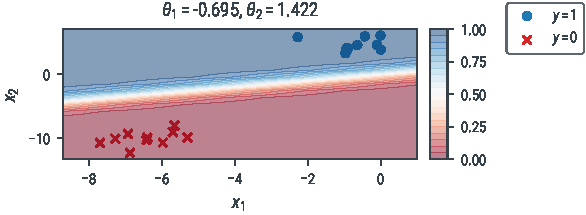
\includegraphics[width=0.7\textwidth]{../figures/bayesian-logistic-regression/mle.pdf}
        \end{figure}
    \end{frame}
}

\MapVsMle{MAP with a weak prior}{100.0}
\MapVsMle{MAP with a medium prior}{1.0}
\MapVsMle{MAP with a strong prior}{0.1}

\section{Fully Bayesian}

\begin{frame}{Posterior}
    \begin{align*}
        p(\boldsymbol{\theta} | \data) & = \frac{p(\data | \boldsymbol{\theta}) p(\boldsymbol{\theta})}{\int p(\data | \boldsymbol{\theta}) p(\boldsymbol{\theta}) d\boldsymbol{\theta}}
    \end{align*}
    \begin{itemize}
        \item Normal prior and Bernoulli likelihood do not form a conjugate pair. Thus, the denominator is intractable and we cannot find the posterior in closed form.
              \pause
        \item We need another method to find the posterior.
              \pause
        \item Laplace approximation!
    \end{itemize}
\end{frame}

\section{Laplace Approximation}

\begin{frame}{A Quick Refresher}
    \begin{align*}
        \text{Neg. Log Joint } f(\theta)                 & = -\log p(\data | \theta) - \log p(\theta)                                                                                                                                                             \\
                                                         & = -\sum_{i=1}^N y_i \log \boldsymbol{\sigma}\left(\boldsymbol{\theta}^T\boldsymbol{x}_i\right) + (1 - y_i) \log \left(1 - \boldsymbol{\sigma}\left(\boldsymbol{\theta}^T\boldsymbol{x}_i\right)\right) \\
                                                         & \quad  - \left( - \frac{1}{2} \frac{\boldsymbol{\theta}^T\boldsymbol{\theta}}{\sigma^2} - \frac{1}{2}\log (2 \pi \sigma^2)\right)                                                                      \\
        \text{Laplace Posterior } q(\boldsymbol{\theta}) & = \mathcal{N}(\theta | \theta_{\text{MAP}}, \nabla^2 f(\theta_{\text{MAP}})^{-1})                                                                                                                      \\
                                                         & = \mathcal{N}(\theta | \theta_{\text{MAP}}, H^{-1})
    \end{align*}
\end{frame}

\begin{frame}{Predictive distribution}
    \begin{align*}
        \onslide<1->{p(y^*=1| \boldsymbol{x}^*, \data) & = \int p(y^*=1| \boldsymbol{x}^*, \boldsymbol{\theta}) p(\boldsymbol{\theta} | \data) d\boldsymbol{\theta}}     \\
        \onslide<2->{                                  & \approx \int p(y^*=1| \boldsymbol{x}^*, \boldsymbol{\theta}) q(\boldsymbol{\theta}) d\boldsymbol{\theta}}       \\
        \onslide<3->{                                  & = \int \boldsymbol{\sigma}(\boldsymbol{\theta}^T \boldsymbol{x}^*) q(\boldsymbol{\theta}) d\boldsymbol{\theta}} \\
        \onslide<4->{                                  & = \mathbb{E}_{q(\boldsymbol{\theta})}\left(
        \boldsymbol{\sigma}(\boldsymbol{\theta}^T \boldsymbol{x}^*)\right)}                                                                                              \\
        \onslide<5->{                                  & \approx \frac{1}{M} \sum_{i=1}^M \boldsymbol{\sigma}(\boldsymbol{\theta}_i^T \boldsymbol{x}^*)}
    \end{align*}
\end{frame}

\newcommand{\LaplaceVsMAP}[2]{
    \begin{frame}{#1}
        Laplace
        \begin{figure}
            \includegraphics[width=0.7\textwidth]{../figures/bayesian-logistic-regression/map_laplace-#2.pdf}
        \end{figure}
        MAP
        \begin{figure}
            \includegraphics[width=0.7\textwidth]{../figures/bayesian-logistic-regression/map_#2.pdf}
        \end{figure}
    \end{frame}
}

\LaplaceVsMAP{Predictive Distribution with a Weak Prior}{100.0}
\LaplaceVsMAP{Predictive Distribution with a Medium Prior}{1.0}
\LaplaceVsMAP{Predictive Distribution with a Strong Prior}{0.1}

\end{document}